\chapter{Implementare}

\section{Introducere}

Acest capitol descrie implementarea algoritmilor descriși anterior, împreună cu modul în care au fost verificate proprietățile acestora, accentul cazând preponderent pe a doua parte.

\section{Structuri de date}

Implementarea teoremei de înlocuire este realizată în principal în cadrul clasei \textit{Formula}. Atributul \textit{formula} reprezintă o formulă propozițională, iar atributul \textit{n} delimitează limita superioară a valorilor variabilelor din formulă.

Pentru atributul \textit{formula} este utilizat un tip de date inductiv definit în modul următor:
\begin{figure}[H]
    \caption{Tipul FormulaT}
    \label{Tipul FormulaT}

\begin{Verbatim}[fontsize=\small, frame=single,baselinestretch=0.1]
datatype FormulaT = Var(val : int)
                | Not(f1 : FormulaT)
                | And(f1 : FormulaT, f2 : FormulaT)
                | Or(f1 : FormulaT, f2: FormulaT)
                | Implies(f1 : FormulaT, f2 : FormulaT)
                | DImplies(f1 :FormulaT, f2 : FormulaT)
\end{Verbatim}

\end{figure}
Fiecare tip de date din componența FormulaT reprezintă un nod din arborele abstract de sintaxă al formulei propozițioanale:

\begin{itemize}
	\item \textit{Var(p)} reprezintă variabila propozitioanală $p$.
	\item \textit{Not(f1)} reprezintă negația formulei \textit{f1}.
	\item \textit{And(f1, f2)} reprezintă conjuncția formulelor \textit{f1} si \textit{f2}.
	\item \textit{Or(f1, f2)} reprezintă disjuncția formulelor \textit{f1} și \textit{f2}.
	\item \textit{Implies(f1, f2)} reprezintă implicația logică, de la \textit{f1} către \textit{f2}.
	\item \textit{DImplies(f1, f2)} reprezintă echivalența formulelor \textit{f1} si \textit{f2}. Echivalența a doua formule mai este numită și dublă implicație.
\end{itemize}

Astfel, rezultă un arbore în care nodurile interne reprezintă conectori logici și pot avea maximum doi fii, iar frunzele reprezintă variabile propoziționale.

Pentru realizarea transformării sunt necesare patru metode principale. Rezumativ, acestea au următorul comportament:
\begin{enumerate}
	\item Metoda \textit{applyOneRule} primește o formulă \textit{f}. Dacă \textit{f} poate fi transformată utilizând una din cele nouă reguli de echivalență din teorema de înlocuire, atunci metoda returnează formula rezultată, dacă nu, este returnată formula primită la intrare.
	\item Metoda \textit{step} primește o formulă \textit{f} asupra căreia aplică metoda \textit{applyOneRule}. Dacă aceasta nu are niciun efect, atunci rădăcina arborelui formulei \textit{f} este de tip \textit{And}, \textit{Or} sau \textit{Not}, caz în care \textit{step} se propagă, fiind apelată utilizând unul dintre nodurile fiu ale rădăcinii. 
	\item Metoda \textit{stepUntilNoChange} primește ca argument o formulă \textit{f}. Dacă apelul metodei \textit{step} asupra lui \textit{f} realizează o modificare, \textit{stepUntilNoChange} este apelată recursiv utilizând noua formulă. Aceasta se oprește în momentul în care apelarea \textit{step} nu aduce modificări.
	\item Metoda \textit{convert} apelează \textit{stepUntilNoChange} utilizând atributul \textit{formula}, prelucrând ulterior formula într-un format vectorial care poate fi utilizat de alți algoritmi.
\end{enumerate}

\subsection{Metoda \textit{applyOneRule}}

Metoda \textit{applyOneRule} primește 3 parametri:
\begin{enumerate}
\item o formulă \textit{f}
\item \textit{nrOfOrR}, reprezintă numărul de noduri etichetate cu \textit{Or} care au în fiul drept formula \textit{f}
\item \textit{nrOfAndR}, reprezintă numărul de noduri etichetate cu \textit{And} care au în fiul drept formula \textit{f}.
\end{enumerate} 
Ultimii doi parametri sunt folosiți doar în scopul verificării. Metoda returnează formula \textit{r}.

Deoarece formula \textit{f} este reprezentată printr-un tip de date inductiv, sunt parcurse primele două nivele din arborele de sintaxă abstractă pentru a aplica una din cele nouă reguli de echivalență.

Sunt prezente urmatoarele precondiții:
\begin{enumerate}
	\item \textit{nrOfOrR $\geq$ 0};
	\item \textit{nrOfAndR $\geq$ 0};
	\item \textit{validFormulaT(f)};
	\item \textit{variablesUpTo(f, n)};
\end{enumerate}

Justificarea necesității primelor două postcondiții este trivială, acestea reflectă faptul că nu putem avea un număr negativ de noduri în cadrul unui arbore.
A treia adnotare cere ca toate valorile corespunzatoare frunzelor arborelui să fie pozitive, iar a patra cere ca acestea să fie strict mai mici decat \textit{n}.

Metoda asigură validitatea urmatoarelor postcondiții:
\begin{enumerate}
	\item \textit{validFormulaT(f)};
	\item \textit{variablesUpTo(f, n)};
	\item \textit{equivalentFormulas(f, r)};
	\item \textit{terminationCondition(f, r, nrOfOrR, nrOfAndR)}; 
\end{enumerate} 

Primele doua postcondiții, fiind prezente ca și precondiții, asigură că metoda nu alterează variabilele, informația garantată de acestea fiind necesară în cadrul verificării satisfiabilității.

A treia postcondiție verifică definiția echivalenței a două formule logice. Aceasta iterează prin toate asignările de mărime \textit{n} si verifică dacă \textit{f} și \textit{r} au aceeași valoare de adevăr. Predicatul poate fi descris formal, în modul următor:
\begin{center}
$\forall assignment : seq<bool>$, $|assignment| = n \Rightarrow$ $truthValueOf(f) = truthValueOf(f)$.
\end{center}

Ultima postcondiție este necesară pentru a demonstra terminarea apelului recursiv al metodei \textit{stepUntilNoChange}. Fiind cea mai complexă adnotare din cadrul lucrării prezente, aceasta va fi descrisă separat impreună cu abordările anterioare care au condus la realizarea ei.

\subsection{Metoda \textit{step}}

Aceasta metodă are aceleași adnotări și date de intrare ca și \textit{applyOneRule}, descrisă anterior. 

In primă instanță este apelată \textit{applyOneRule} folosind formula \textit{f}. Având aceleași adnotări, validitatea precondițiilor se pastrează. Datorită modului în care sunt formulate cele nouă reguli de echivalență, există situații în care este necesară propagarea în cadrul arborelui de sintaxă abstractă. Pentru tipurile \textit{DImplies} și \textit{Implies}, \textit{applyOneRule} are efect întotdeauna, indiferent de fii celor două noduri. Pentru \textit{And, Or} și \textit{Not} există cazuri în care nu putem aplica nicio regulă, iar formula nu este încă în formă normală conjunctivă. Pentru nodurile de tip \textit{Not}, propagarea se realizează utilizând singurul fiu existent. Pentru nodurile de tip \textit{And} și \textit{Or}, se realizează propagarea utilizând fiul stang. Dacă aceasta nu are niciun efect, se repetă pasul anterior utilizând fiul drept. 

Trebuie menționat faptul că atunci când se realizează propagarea utilizând nodul drept al unui nod \textit{Or} variabila \textit{nrOfOrR} este incrementată. Se procedează echivalent și în cazul nodului \textit{And} și al variabilei \textit{nrOfAndR}.

Atunci când transformarea se realizează într-unul din fii nodului rădăcină, proprietățile ce vizează viabilitatea formulei se pastrează. Aceeași proprietate este valabilă și pentru proprietatea de echivalență dintre formula primită și cea rezultată. 

\subsection{Metoda \textit{stepUntilNoChange}}

Spre deosebire de ultimele două metode, \textit{stepUntilNoChange} primește la intrare doar o formulă \textit{f} deoarece aceasta este apelată folosind atributul \textit{formula}. Sunt prezente, în continuare, precondițiile și postcondițiile specifice validității formulei. În cadrul metodei se realizează apelul \textit{step(f, 0, 0)}. În continuare, dacă apelul a modificat formula, \textit{stepUntilNoChange} este apeleată din nou, utilizând rezultatul obținut. În caz contrar, execuția se opreste. 

Deoarece nu există nicio garanție că recursia menționată anterior se termină, aceasta trebuie descrisă într-o adnotare a metodei. Această adnotare creează nevoia adăugării predicatului \textit{terminationCondition} ca și postcondițiile metodelor \textit{applyOneRule} și \textit{step}. Dată fiind complexitatea acestui predicat, acesta va fi descris într-o secțiune separată.

\section{Algoritm verificat pentru aducerea unei formule in CNF}

Pentru a realiza conversia atributului \textit{formula} este necesar apelul metodei \textit{convert}:

\begin{figure}[H]
    \caption{Metoda \textit{convert}}

\begin{Verbatim}[fontsize=\small, frame=single,baselinestretch=0.1]
method convert() returns (r : seq<seq<int>>)
  modifies this;
  requires valid();
  ensures valid();
  ensures old(n) == n;
  ensures equivalentFormulas(formula, old(formula));
{
  var formula' := stepUntilNoChange(formula);
  assert equivalentFormulas(formula, formula');

  formula := formula';
}
\end{Verbatim}
\end{figure}

Precondiția \textit{valid} este garantată de constructor, care validează parametrii primiți la instanțierea clasei. Deoarece metoda \textit{convert} pastrează valoarea de adevăr a predicatului \textit{valid}, acesta din urmă este satisfăcut pe durata întregii execuții a programului. Predicatul \textit{valid} reprezintă apelul predicatelor \textit{validFormulaT} și \textit{variablesUpTo} utilizând atributele clasei.

Metoda garantează că atributul \textit{n} nu este modificat, prin postcondiția \textit{old(n) == n}. Totodată, este asigurată echivalența între starea \textit{formulei} de dinainte și respectiv de după execuția metodei.

Pentru realizarea conversiei, este folosită metoda \textit{stepUntilNoChange}.

\begin{figure}[H]
    \caption{Metoda \textit{stepUntilNoChange}}

\begin{Verbatim}[fontsize=\small, frame=single,baselinestretch=0.1]
method stepUntilNoChange(f : FormulaT) returns (r : FormulaT)
  decreases countAndUnderOr(f);
  decreases countDImplies(f);
  decreases countImplies(f);
  decreases countOrOr(f, 0);
  decreases countAndAnd(f, 0);
  requires validFormulaT(f);
  requires variablesUpTo(f, n);
  ensures validFormulaT(r);
  ensures variablesUpTo(r, n);
  ensures equivalentFormulas(f, r);
{
  var res := step(f, 0, 0);

  if(res != f) {
    r := stepUntilNoChange(res);
  }
  else {
    r := res;
  }
}
\end{Verbatim}
\end{figure}

Este apelată metoda \textit{step}, descrisă în sectiunea anterioară. Dacă acest apel realizează modificări asupra parametrului \textit{f}, execuția se reia utilizând noua formulă. În caz contrar, execuția se oprește. Validitatea postcondițiilor este garantată de către apelul step.

\begin{figure}[H]
    \caption{Implementarea metodei \textit{step} pentru propagarea sub nodul \textit{And}}
    

\begin{Verbatim}[fontsize=\small, frame=single,baselinestretch=0.1]
method step(f : FormulaT, nrOfOrR : int, nrOfAndR : int) 
       returns (r : FormulaT)
  decreases f;
  requires nrOfOrR >= 0;
  requires nrOfAndR >= 0;
  requires validFormulaT(f);
  requires variablesUpTo(f, n);
  ensures validFormulaT(r);
  ensures variablesUpTo(r, n);
  ensures equivalentFormulas(f, r);
  ensures terminationCondition(f, r, nrOfOrR, nrOfAndR);
{
  var res : FormulaT := applyOneRule(f, nrOfOrR, nrOfAndR);

  if(f.And? && res == f)
  {
    var f1_step := step(f.f1, nrOfOrR, nrOfAndR);
            
    if (f.f1 == f1_step)
    {
      var f2_step := step(f.f2, nrOfOrR, nrOfAndR + 1);
      res := And(f.f1, f2_step);
      return res;
    }
    else
    {
      res := And(f1_step, f.f2);
      return res;
    }
  }
}

\end{Verbatim}
\end{figure}

În cadrul implementării de mai sus, \textit{applyOneRule} este apelată utilizând parametrii metodei. Dacă apelul nu modifică formula, se incearcă în primă fază propagarea metodei \textit{step} utilizând fiul stang. Dacă formula nu este modificată, se realizează propagarea folosind fiul drept. Abordarea este similară în cazul nodurilor de tip \textit{Or} și \textit{Not}.
În unele cazuri, deoarece modificăm unul dintre fii, este necesară utilizarea lemelor pentru a demonstra validitatea predicatului \textit{terminationCondition}.

\begin{figure}[H]
    \caption{Implementarea metodei \textit{applyOneRule}, doar pentru prima echivalență.}
    
\begin{Verbatim}[fontsize=\small, frame=single,baselinestretch=0.1]
method applyOneRule(f : FormulaT, nrOfOrR : int, nrOfAndR : int) 
       returns (r : FormulaT)
  decreases f;
  requires nrOfOrR >= 0;
  requires nrOfAndR >= 0;
  requires validFormulaT(f);
  requires variablesUpTo(f, n);
  ensures validFormulaT(r);
  ensures variablesUpTo(r, n);
  ensures equivalentFormulas(f, r);
  ensures terminationCondition(f, r, nrOfOrR, nrOfAndR);
{
  match f
  {
    case DImplies(f1, f2) => 
    { 
      r := And(Implies(f1, f2), Implies(f2, f1));
      Rule1Prop1(f1, f2);
      Rule3Const1(f1, f2);
    }
    case Implies(f1, f2) => { r := f;}
    case And(f1, f2)     => { r := f;}
    case Or(f1, f2)      => { r := f;}
    case Var(val)        => { r := f;}
    case Not(f1)         => { r := f;}
   }
}
\end{Verbatim}
\end{figure}

Metoda \textit{applyOneRule} aplică, asupra formulei \textit{f}, una din cele nouă reguli de echivalență, dacă este posibil. În caz contrar, formula este returnată fără modificări.

Aici este punctul de plecare al verificării echivalenței formulelor. Pentru fiecare din cele nouă echivalențe, putem verifica faptul că \textit{f} și \textit{r} au aceeași valoare de adevăr în orice asignare a celor \textit{n} variabile:

\begin{figure}[H]
    \caption{Implementarea predicatului \textit{equivalentFormulas}.}
\begin{Verbatim}[fontsize=\small, frame=single,baselinestretch=0.1]
predicate equivalentFormulas(f1: FormulaT, f2: FormulaT)
  reads `n;
  requires variablesUpTo(f1, n);
  requires variablesUpTo(f2, n);
  requires validFormulaT(f1);
  requires validFormulaT(f2);
  {
    forall assignment : seq<bool> ::  |assignment| == n ==> 
     truthValueOfF(f1, assignment) == truthValueOfF(f2, assignment)
  }
\end{Verbatim}
\end{figure}

\begin{remark}
Predicatul \textit{truthValueOF} returnează valoarea de adevăr a unei formule utilizând o anumită asignare a variabilelor propoziționale.
\end{remark}

Demonstrarea terminării execuției programului, asigurată de predicatul \textit{terminationCondition}, va fi descrisă în secțiunea următoare.



\section{Demonstrarea terminării}


În cadrul limbajului de programare Dafny se poate demonstra că execuția unei funcții sau metode recursive se termină, utilizând adnotări de descreștere, conform descrierii din secțiunea \ref{Condiții de terminare}.

\begin{remark}
Precizarea regulilor de echivalență utilizate se va realiza utilizând numerotarea din secțiunea \ref{reguli}.
\end{remark} 

Condiția necesară pentru a verificarea terminării recursiei din cadrul funcției \textit{stepUntilNoChange} este exprimată folosind cinci funcții. Fiecare funcție primește o formulă propozițională și returnează o valoare pozitivă ce exprimă o anumită proprietate a formulei.   

\subsubsection{Funcția \textit{countImplies}}

Funcția \textit{countImplies}, fiind și cea mai simplă, parcurge arborele de sintaxă abstractă și numară nodurile etichetate cu simbolul $\Rightarrow$. Funcția calculează o expresie pe baza arborelui formulei, unde fiecare nod $\Rightarrow$ are valoarea 1. 

\subsubsection{Funcția \textit{countDImplies}}

Spre deosebire de \textit{countImplies}, funcția în cauză trebuie să facă o diferențiere între nodurile de tipul \textit{DImplies}. 

În cadrul expresiei, valoarea unui nod "$\Leftrightarrow$" crește exponențial în funcție de valoarea returnată în urma evaluării fiilor săi:
\begin{center}
\textit{countDImplies($\varphi_1$, $\varphi_2)$ = $2^{countDImplies(\varphi_1) + countDImplies(\varphi_2)} + 1$}.
\end{center}
\subsubsection{Funcțiile \textit{countOrOr} și \textit{countAndAnd}}

În cadrul calculului realizat de funcția \textit{countOrOr}, fiecare nod "$\lor$" adaugă la suma rezultată numarul de noduri "$\lor$" în al caror fiu drept se află.
Cu alte cuvinte, \textit{countOrOr} numara de câte ori un nod "$\lor$" apare în fiul drept al unui nod "$\lor$". Funcția primește un argument numeric suplimentar, \textit{nrOfOrR}, inițializat cu 0. Funcția parcurge arborele formulei și adună la rezultat parametrul \textit{nrOfOrR} de fiecare dată când evaluează un nod de tip "$\lor$". La fiecare propagare în fiul drept al unui nod de tip "$\lor$", \textit{nrOfOrR} este incrementat. 

Funcția \textit{countAndAnd} are comportamentul descris mai sus, cu precizarea ca utilizează nodurile de tip "$\land$".

\subsubsection{Funcția \textit{countAndUnderOr}}

Funcția \textit{countAndUnderOr}, fiind și cea mai complexă, este utilizată pentru a verifica terminarea aplicării a cinci dintre cele nouă reguli de echivalență. În cadrul acesteia, nodurile de tip \textit{Var} și "$\land$" au o influență lineară asupra rezultatului în timp ce nodurile \textit{Not} aduc o creștere exponentială. Nodurile de tip "$\lor$" returnează înmultirea dintre rezultatele evaluării fiilor. Arborii ce au ca radacină noduri de tipul "$\Leftrightarrow$" sau "$\Rightarrow$" sunt evaluați utilizând echivalențele corespunzatoare primelor două reguli de echivalență.

\begin{figure}[H]
\centering
\caption{Implementarea countAndUnderOr în Dafny}
\begin{Verbatim}[fontsize=\small, frame=single,baselinestretch=0.1]
function countAndUnderOr(f : FormulaT) : (res : int)
decreases f;
ensures res >= 2;
{
  match f
  {
    case Var(val)         => 2
    case Not(f1)          => pow(2, countAndUnderOr(f1))
    case And(f1, f2)      => 
      countAndUnderOr(f1) + countAndUnderOr(f2) + 1
    case Or(f1, f2)       => 
      countAndUnderOr(f1) * countAndUnderOr(f2)
    case Implies(f1, f2)  => 
      pow(2, countAndUnderOr(f1)) * countAndUnderOr(f2)
    case DImplies(f1, f2) => 
      (pow(2, countAndUnderOr(f1)) * countAndUnderOr(f2)) + 
      (pow(2, countAndUnderOr(f2)) * countAndUnderOr(f1)) + 1
  }
}
\end{Verbatim} 

Următoarea ordonare a funcțiilor respectă precizările din secțiunea \ref{Condiții de terminare}:
\begin{enumerate}
\item \textit{countAndUnderOr};
\item \textit{countDImplies};
\item \textit{countImplies};
\item \textit{countOrOr};
\item \textit{countAndAnd}; 
\end{enumerate}   

\end{figure}

Fie $f_1, f_2, ..., f_5$ etichetarea funcțiilor menționate anterior și $\varphi_i$' formula obținută în urma aplicării regulii $i$ asupra formulei $\varphi_i$. În cazul de fată, pentru verificarea terminării recursiei, trebuie indeplinită urmatoarea proprietate: $\forall i \in [1, 9], \exists j \in [1, 5]$ astfel încât $f_j(\varphi_j') < f_j(\varphi_j)$ și $\forall k \in [1,j - 1], f_k(\varphi_k\\mathaccent) \leq f_k(\varphi_k),$ unde $i, j, k \in \mathbb{N}.  $

În continuare, este descris modul in care este modificată formula în urma aplicării fiecarei echivalențe, explicitând proprietatea enuntată anterior.

\begin{remark}
Partea stangă a echivalențelor va fi notată cu $\varphi$, iar partea dreaptă cu $\varphi$'.
\end{remark} 

\subsubsection{Echivalența 1}

Prima echivalență elimină implicațiile duble: $( \varphi_1 \Leftrightarrow \varphi_2) \equiv ((\varphi_1 \Rightarrow \varphi_2) \land (\varphi_2 \Rightarrow \varphi_1)).$

Transformarea formulei poate fi vizualizată mai ușor utilizând arbori:

\begin{figure}[H]
\caption{Echivalența 1}
\centering
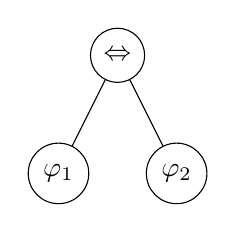
\begin{tikzpicture}[
    tlabel/.style={pos=0.4,right=-1pt},
    baseline=(current bounding box.center)
    ]
	\node [circle, draw]{$\Leftrightarrow$}
		child{node [circle, draw]{$\varphi_1$}}
		child{node [circle, draw]{$\varphi_2$}}
;
  \end{tikzpicture}
  $\Rightarrow$ % the arrow between the pictures
  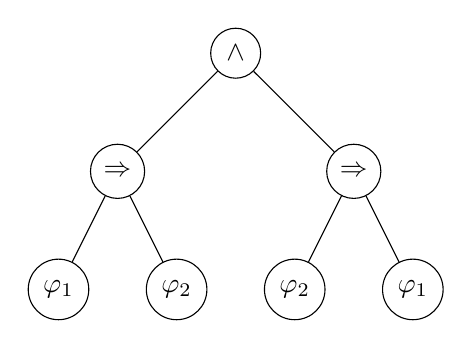
\begin{tikzpicture}[
    tlabel/.style={pos=0.4,right=-1pt},
    baseline=(current bounding box.center),
    level 1/.style={sibling distance=30mm},
    level 2/.style={sibling distance=15mm}
    ]
	\node [circle, draw]{$\land$}
		child{node [circle, draw]{$\Rightarrow$}
			child{node [circle, draw]{$\varphi_1$}}
			child{node [circle, draw]{$\varphi_2$}}
		}
		child{node [circle, draw]{$\Rightarrow$}
			child{node [circle, draw]{$\varphi_2$}}
			child{node [circle, draw]{$\varphi_1$}}			
		}
;
  \end{tikzpicture}
  
\end{figure}

Funcția a cărei valoare descrește în cazul acestei echivalențe este \textit{countDImplies}:
\begin{align*}
	countDImplies(\varphi') &<
		countDImplies(\varphi) \\
	countDImplies(Implies(\varphi_1, \varphi_2)) + & \\
    countDImplies(Implies(\varphi_2, \varphi_1) &< 
    	 1 + 2 ^ {countDImplies(\varphi_1) + countDImplies(\varphi_2)} \\
    2 * ( countDImplies(\varphi_1) + countDImplies(\varphi_2)) &< 
    	1 + 2 ^ {countDImplies(\varphi_1) + countDImplies(\varphi_2)} 
\end{align*}

\begin{remark}
$\forall x \geq 0, x * 2 < 1 + 2 ^ x.$
\end{remark}

Singura funcție care precede \textit{countDImplies} este \textit{countAndUnderOr}. Se observă din implementarea funcției că: $countAndUnderOr(\varphi') = countAndUnderOr(\varphi)$.

\subsubsection{Echivalența 2}

Echivalența 2 elimină implicațiile simple: $(\varphi_2 \Rightarrow \varphi_1) \equiv (\neg \varphi_1 \lor \varphi_2)$.

\begin{figure}[H]
\caption{Echivalența 2}
\centering
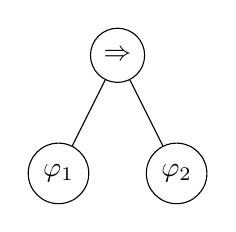
\begin{tikzpicture}[
    tlabel/.style={pos=0.4,right=-1pt},
    baseline=(current bounding box.center)
    ]
	\node [circle, draw]{$\Rightarrow$}
		child{node [circle, draw]{$\varphi_1$}}
		child{node [circle, draw]{$\varphi_2$}}
;
  \end{tikzpicture}
  $\Rightarrow$ % the arrow between the pictures
  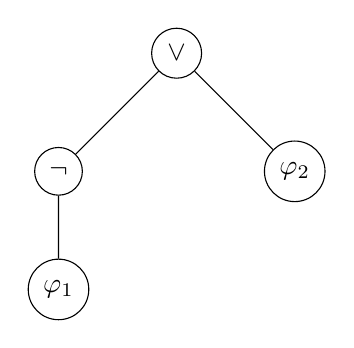
\begin{tikzpicture}[
    tlabel/.style={pos=0.4,right=-1pt},
    baseline=(current bounding box.center),
    level 1/.style={sibling distance=30mm},
    level 2/.style={sibling distance=15mm}
    ]
	\node [circle, draw]{$\lor$}
		child{node [circle, draw]{$\neg$}
			child{node [circle, draw]{$\varphi_1$}}
		}
			child{node [circle, draw]{$\varphi_2$}}
;
  \end{tikzpicture}
  
\end{figure}

Funcția a cărei valoare descrește în cazul acestei echivalențe este \textit{countImplies}:
\begin{align*}
	countImplies(\varphi') &< countImplies(\varphi) \\
	countDImplies(\varphi_1) + countImplies(\varphi_2) &< countImplies(\varphi_1) + countImplies(\varphi_2) + 1 \\
\end{align*} 

Funcțiile care preced \textit{countImplies} sunt \textit{countAndUnderOr} și \textit{countDImplies}. Se observă din implementarea funcțiilor că: 
\begin{itemize}
\item $countAndUnderOr(\varphi') = countAndUnderOr(\varphi)$;
\item $countDImplies(\varphi') = countDImplies(\varphi)$;
\end{itemize} 

\subsubsection{Echivalențele 3 și 4}

Echivalențele 3 și 4 asigură faptul că în arborele formulei toate disjuncțiile "coboară" sub conjuncții: 
\begin{itemize}
\item $(\varphi_1 \lor (\varphi_2 \land \varphi_3)) \equiv ((\varphi_1 \lor \varphi_2) \land (\varphi_1 \lor \varphi_3));$
\item $((\varphi_2 \land \varphi_3) \lor \varphi_1) \equiv ((\varphi_2 \lor \varphi_1) \land (\varphi_3 \lor \varphi_1));$ 
\end{itemize}

Deoarece descrierea regulilor este similară, va fi explicitat doar comportamentul echivalenței $3$. Fie $a, b, c$ valorile returnate de apelurile \textit{countAndUnderNot($\varphi_1$)}, \textit{countAndUnderNot($\varphi_2$)} și \textit{countAndUnderNot($\varphi_3$)}.

\begin{figure}[H]
\caption{Echivalența 3}
\centering
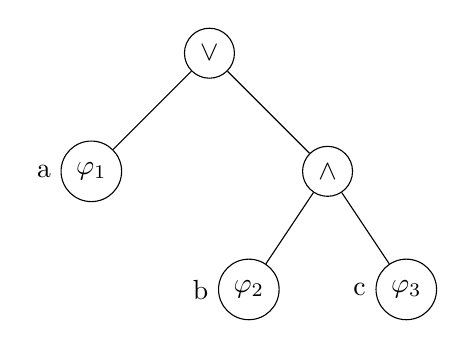
\begin{tikzpicture}[
    tlabel/.style={pos=0.4,right=-1pt},
    baseline=(current bounding box.center),
    level 1/.style={sibling distance=30mm},
    level 2/.style={sibling distance=20mm}    
    ]
	\node [circle, draw]{$\lor$}
		child{node [circle, draw, label = left:{a}]{$\varphi_1$}}
		child{node [circle, draw]{$\land$}
			child{node [circle, draw, label = left:{b}]{$\varphi_2$}}
			child{node [circle, draw, label = left:{c}]{$\varphi_3$}}
		}
;
  \end{tikzpicture}
  $\Rightarrow$ % the arrow between the pictures
  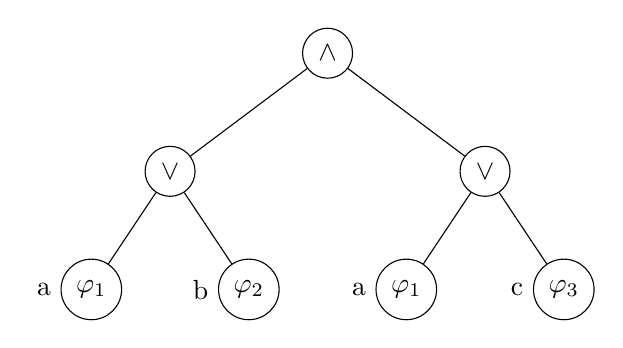
\begin{tikzpicture}[
    tlabel/.style={pos=0.4,right=-1pt},
    baseline=(current bounding box.center),
    level 1/.style={sibling distance=40mm},
    level 2/.style={sibling distance=20mm}
    ]
	\node [circle, draw]{$\land$}
		child{node [circle, draw]{$\lor$}
			child{node [circle, draw, label = left:{a}]{$\varphi_1$}}
			child{node [circle, draw, label = left:{b}]{$\varphi_2$}}
		}
		child{node [circle, draw]{$\lor$}
			child{node [circle, draw, label = left:{a}]{$\varphi_1$}}
			child{node [circle, draw, label = left:{c}]{$\varphi_3$}}
		}
;
  \end{tikzpicture}
\end{figure}

Funcția a cărei valoare descrește strict în cazul acestei echivalențe este \textit{countAndUderOr}. 




\begin{align*}
	countAndUnderNot(\varphi') &< countAndUnderNot(\varphi) \\
	a * b + a * c + 1  &< a * (b + c + 1) \\
	a * b + a * c + 1  &< a * b + a * c + a \\
		1 &< a
\end{align*}

Funcția \textit{countAndUnderNot} garantează printr-o postcondiție că rezultatul este mai mare decât $1$. În cadrul evaluării, nodurile frunză au valoarea $2$, iar valoarea rezultată în urma evaluării nodurilor interne este intotdeauna mai mare decât valoarea evaluării fiilor. 

\subsubsection{Echivalența 5}

Echivalența 5 vizează asociativitatea lanțurilor de disjuncții, pentru a permite scrierea $\varphi_1 \lor \varphi_2 \lor  . . . \lor \varphi_n$ în loc de
$(((\varphi_1 \lor \varphi_2) \lor  . . .) \lor \varphi_n)$:
\begin{center}
$(\varphi_1 \lor (\varphi_2 \lor \varphi_3)) \equiv ((\varphi_1 \lor \varphi_2) \lor \varphi_3))$.
\end{center} 

Funcția a cărei valoare descrește în cazul echivalenței 5 este \textit{countOrOr}.

\begin{figure}[H]
    \caption{Implementarea funcției \textit{countOrOr}.}
\begin{Verbatim}[fontsize=\small, frame=single,baselinestretch=0.1]
function countOrOr(f : FormulaT, nrOfOrR : int) : (res : int)
 decreases f;
 requires nrOfOrR >= 0;
 ensures res >= 0;
{
  match f
 {
   case Or(f11,f12)       => 
     countOrOr(f11, nrOfOrR) + countOrOr(f12, nrOfOrR + 1) + nrOfOrR
   case And(f11,f12)      => 
     countOrOr(f11, nrOfOrR) + countOrOr(f12, nrOfOrR)
   case Var(val)          => 0
   case Implies(f11,f12)  => 
     countOrOr(f11, nrOfOrR) + countOrOr(f12, nrOfOrR)
   case DImplies(f11,f12) => 
     countOrOr(f11, nrOfOrR) + countOrOr(f12, nrOfOrR)
   case Not(f1)           => countOrOr(f1, nrOfOrR)
 }
}
\end{Verbatim}
\end{figure}

Fie $x$ valoarea parametrului \textit{nrOfOrOr} în nodul radacină, reprezentând numărul de noduri "$\lor$" în al căror fiu drept se află formula. Valorile returnate de apelurile  \textit{countOrOr($\varphi_1$, nrOfOrOr)}, \textit{countOrOr($\varphi_2$, nrOfOrOr+1)}, \textit{countOrOr($\varphi_3$, nrOfOrOr+1)} și \textit{countOrOr($\varphi_3$, nrOfOrOr)} vor fi notate cu $a, b, c$ și respectiv $c'$. Se observă că $c' < c$.


\begin{figure}[H]
\caption{Echivalența 5}
\centering
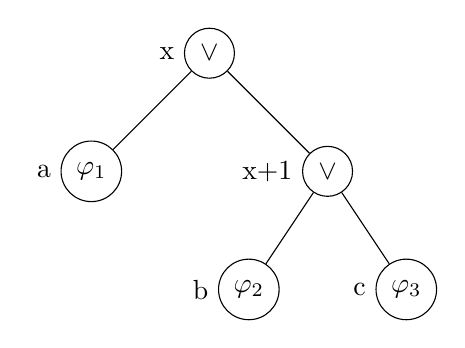
\begin{tikzpicture}[
    tlabel/.style={pos=0.4,right=-1pt},
    baseline=(current bounding box.center),
        level 1/.style={sibling distance=30mm},
    level 2/.style={sibling distance=20mm}
    ]
	\node [circle, draw, label = left:{x}]{$\lor$}
		child{node [circle, draw, label = left:{a}]{$\varphi_1$}}
		child{node [circle, draw, label = left:{x+1}]{$\lor$}
			child{node [circle, draw, label = left:{b}]{$\varphi_2$}}
			child{node [circle, draw, label = left:{c}]{$\varphi_3$}}			
		}
;
  \end{tikzpicture}
  $\Rightarrow$ % the arrow between the pictures
  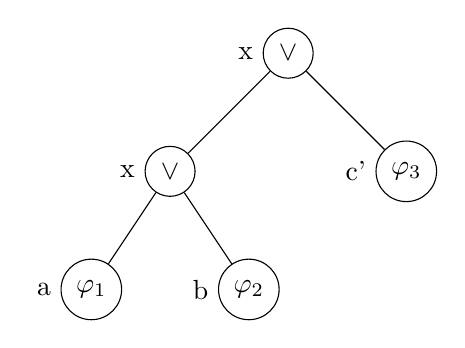
\begin{tikzpicture}[
    tlabel/.style={pos=0.4,right=-1pt},
    baseline=(current bounding box.center),
    level 1/.style={sibling distance=30mm},
    level 2/.style={sibling distance=20mm}
    ]
	\node [circle, draw, label = left:{x}]{$\lor$}
		child{node [circle, draw, label = left:{x}]{$\lor$}
			child{node [circle, draw, label = left:{a}]{$\varphi_1$}}
			child{node [circle, draw, label = left:{b}]{$\varphi_2$}}			
		}
		child{node [circle, draw, label = left:{c'}]{$\varphi_3$}}

;
  \end{tikzpicture}
  
\end{figure}

Valoarea returnată de funcția \textit{countOrOr} scade strict:

\begin{align*}
	countOrOr(\varphi') &< countOrOr(\varphi) \\
	x + x + c' + a + b  &< x + a + x + 1 + b + c \\
	\cancel{x} + \cancel{x} + c' + \cancel{a} + \cancel{b}  &< \cancel{x} + \cancel{a} + \cancel{x} + 1 + \cancel{b} + c \\
	c'  &< c + 1
\end{align*}

In cadrul condiției de terminare, funcția \textit{countOrOr} este precedată de \textit{countAndUnderNot}, \textit{countDImplies} și \textit{countImplies}. Valoarea acestora nu se modifică, în cazul acestei transformări, datorită asociativității operațiilor de înmulțire (pentru prima funcție) și respectv adunare (pentru ultimele două).

\subsubsection{Echivalența 6}

Echivalența 6 vizează asociativitatea lanțurilor de conjuncții, pentru a permite scrierea $\varphi_1 \land \varphi_2 \land  . . . \land \varphi_n$ în loc de
$(((\varphi_1 \land \varphi_2) \land  . . .) \land \varphi_n)$:
\begin{center}
$(\varphi_1 \land (\varphi_2 \land \varphi_3)) \equiv ((\varphi_1 \land \varphi_2) \land \varphi_3))$.
\end{center}

Comportamentul este similar cu cel al echivalenței abordate anterior, cu precizarea că sunt vizate conjuncțiile în loc de disjuncții.

Funcția a cărei valoare descrește în urma aplicării acestei reguli este \textit{countOrOr}. La fel ca și la echivalența 5, valoarile returnate de primele trei functii din enumerarea condiției de terminare nu se modifică. Funcția \textit{countOrOr} nu iși modifică valoarea deoarece transformarea nu modifică numărul de disjuncții din dreapta nodurilor de tip "$\lor$".

\begin{remark}
În cadrul condiției de terminare, ordinea funcțiilor \textit{countOrOr} și \textit{countAndAnd} este irelevantă deoarece echivalențele vizate de către acestea sunt independente. Regula 5 nu modifică valoarea funcției care vizeaza regulă 6, și invers. 
\end{remark}

\subsubsection{Echivalențele 7 și 8}

Echivalențele 7 si 8 asigură faptul că, în cadrul arborelui formulei, toate negațiile "coboară" sub conjuncții si disjuncții:
\begin{itemize}
\item $\neg (\varphi_1 \lor \varphi_2) \equiv (\neg \varphi_1 \land \neg \varphi_2);$
\item $\neg (\varphi_1 \land \varphi_2) \equiv (\neg \varphi_1 \lor \neg \varphi_2);$
\end{itemize}


Deoarece efectul regulilor este similar, va fi explicitat doar comportamentul echivalenței 7. 


\begin{figure}[H]
\caption{Echivalența 7}
\centering
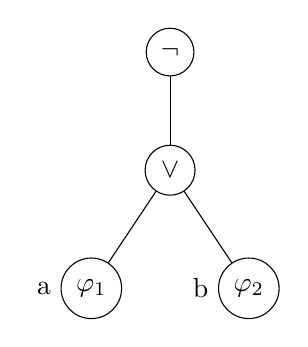
\begin{tikzpicture}[
    tlabel/.style={pos=0.4,right=-1pt},
    baseline=(current bounding box.center),
        level 1/.style={sibling distance=30mm},
    level 2/.style={sibling distance=20mm}
    ]
	\node [circle, draw]{$\neg$}
		child{node [circle, draw]{$\lor$}
			child{node [circle, draw, label = left:{a}]{$\varphi_1$}}
			child{node [circle, draw, label = left:{b}]{$\varphi_2$}}			
		}
;
  \end{tikzpicture}
  $\Rightarrow$ % the arrow between the pictures
  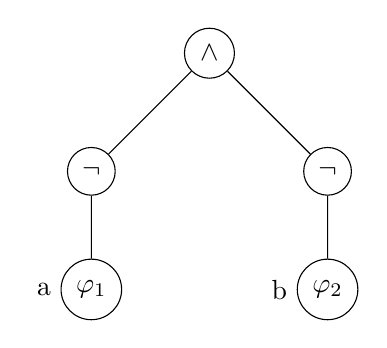
\begin{tikzpicture}[
    tlabel/.style={pos=0.4,right=-1pt},
    baseline=(current bounding box.center),
    level 1/.style={sibling distance=30mm},
    level 2/.style={sibling distance=20mm}
    ]
	\node [circle, draw]{$\land$}
		child{node [circle, draw]{$\neg$}
			child{node [circle, draw, label = left:{a}]{$\varphi_1$}}		
		}
		child{node [circle, draw]{$\neg$}
			child{node [circle, draw, label = left:{b}]{$\varphi_2$}}		
		}
;
  \end{tikzpicture}
  
\end{figure}

Funcția a cărei valoare descreste în urma aplicării regulii 7 este \textit{countAndUnderOr}. Fie $a$ si $b$ valorile apelurilor \textit{countAndUnderOr($\varphi_1$)} și respectiv \textit{countAndUnderOr($\varphi_1$)}.

\begin{align*}
	countAndUnderNot(\varphi') &< countAndUnderNot(\varphi) \\
	2^a + 2^b + 1 &< 2^{a*b} \\
\end{align*}

\begin{remark}
Inecuatia de mai sus este demonstrată în cadrul implementării utilizând leme pentru $\forall a, b \geq 2$, unde $a, b \in \mathbb{N}$.
\end{remark}

O abordare mai eficientă din punct de vedere computațional este implementarea unei funcții care numară conjuncțiile și disjuncțiile de sub fiecare nod de tip "$\neg$".

\subsubsection{Echivalența 9}

Ultima echivalentă asigură că nu există două negații "imediat una sub alta" în arborele de sintaxă abstractă al formulei: $\neg \neg \varphi \equiv \varphi.$

Funcția a cărei valoare descrește în urma aplicării acestei echivalențe este \textit{countAndUnderOr}.
\begin{align*}
	countAndUnderNot(\varphi') &< countAndUnderNot(\varphi) \\
	2^{2^{countAndUnderNot(\varphi)}} &< countAndUnderNot(\varphi)\\
\end{align*}

O abordare mai e eficientă din punct de vedere computațional este implementarea unei funcții care numară nodurile de tip "$\neg$".



